\fancychapter{Implementation}
\label{chap:imp}
\textcolor{red}{introdução do capítulo}





\section{DC-DC converter}
\textcolor{red}{introdução do capítulo}

\subsection{Operation principles}
The DC-DC converter chosen for this project was a boost converter. This topology uses one switching device, one inductor, one output capacitor and a diode, Figure \ref{fig:boost}. The switching device is used to control the output voltage by switching on and off at a specified frequency (fsw) and duty cycle (D). The inductor is used to store energy when the switch is on (stage 1) and release it when the switch is off (stage 2), while the output capacitor is used to smooth the output voltage, Figure~\ref{fig:boost}.

\begin{figure}[!ht]
    \centering
    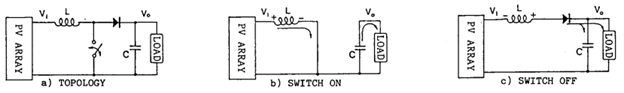
\includegraphics[width=0.9\textwidth]{Images/Implementation/Boost.png}
    \caption{Classic Boost converter topology and stages \cite{Comparison_PV_Converter_Technologies_1989}.}
    \label{fig:boost}
\end{figure}

Analyzing the boost converter separately on his two stages, it is possible to define the drop  voltage across the inductor (VL), as a function of the input voltage (Vin) and output voltage (Vout) as follows:

\begin{equation}
    V_L = \begin{cases}
    V_{in} & \text{if } t \in [0, D \cdot T] \\
    V_{in} - V_{out} & \text{if } t \in [D \cdot T, T]
  \end{cases}
  \label{eq:vl}
\end{equation}

With equation \ref{eq:vl} and the fact that at stationary state the average voltage across the inductor is zero, it is possible to define the output voltage in function of the input voltage and duty cycle as follows:

\begin{equation}
    V_{Lavg} = \frac{1}{T} (\int_{0}^{DT} V_{in} dt + \int_{DT}^{T} (V_{in} - V_{out}) dt) = 0 \Rightarrow V_{out} = \frac{V_{in}}{1-D}
    \label{eq:duty}
\end{equation}

Equation \ref{eq:duty} is one of the most important equations in boost converter design, as it defines the relationship between the input voltage, output voltage and duty cycle. As the duty cycle increases, the output voltage also increases, which is the main principle behind boost converters. For our use case, it is import to analyze the relation between the input and output current as well. Considering no power losses, it is possible to define the input current as follows:
\begin{equation}
    P_{in} = P_{out} \Leftrightarrow V_{in} \cdot I_{in} = V_{out} \cdot I_{out} \Leftrightarrow I_{in} = \frac{V_{out}}{V_{in}} \cdot I_{out} \Leftrightarrow I_{in} = \frac{I_{out}}{1-D}
\end{equation}

However, these equations are only valid for ideal components since it does not take into account the parasitic elements of the components, such as the resistance of the inductor, the drain source resistance of the transistor, and the voltage drop across the diode (there are more parasitic components that affect the performance). In a real boost converter, these parasitic elements will cause a voltage drop and therefore reduce the output voltage. 

Let's quickly analyze the influence of the inductor resistance ($R_L$) and the voltage drop across the diode ($V_d$) by changing the equation \ref{eq:vl} to:

\begin{equation}
    V_L = \begin{cases}
    V_{in} - R_{DS_{(on)}} \cdot I_{DS} & \text{if } t \in [0, D \cdot T] \\
    V_{in} - V_{out} - V_d & \text{if } t \in [D \cdot T, T]
  \end{cases}
  \label{eq:vl2}
\end{equation}

In this case the at stationary state the average voltage across the inductor is $R_L \cdot I_L$ and therefore the output voltage can be defined as:

\begin{equation}
    V_{Lavg} = \frac{1}{T} (\int_{0}^{DT} (V_{in} - R_{DS_{(on)}} \cdot I_{DS}) dt + \int_{DT}^{T} (V_{in} - V_{out} - V_d) dt) \Leftrightarrow 
\end{equation}

\begin{equation}
    \Leftrightarrow R_L \cdot I_L = \frac{1}{T} [T \cdot D \cdot  (V_{in} - R_{DS_{(on)}} \cdot I_{DS}) + T \cdot (1-D)\cdot(V_{in} - V_{out} -V_d)] \Leftrightarrow  V_{out} = \frac{V_{in} - R_{DS_{(on)}} \cdot I_{DS} - R_L \cdot I_L}{1-D}-V_d
    \label{eq:vout2}
\end{equation}

Equation \ref{eq:vout2} shows the 3 mains causes of losses in a boost converter. The main cause is the voltage drop across the diode, which causes a significant reduction in the output voltage (usually 0.3~V to 0.7~V). This will be solved by using a synchronous boost converter (Figure~\ref{fig:sync_boost}), which replaces the diode with a transistor. In synchronous boost converters the voltage drop across the transistor is much smaller due to the low $R_{DS,on}$, usually lower than 0.1~V.

As for the inductor internal resistance, it is not possible to remove it entirely, so it must be taken into account when designing the boost converter. The same is true for the drain source resistance of the transistor, which is also not possible to remove entirely. Therefore, it is important to select components with low internal resistance to minimize the losses and increase the efficiency of the converter.

\begin{figure}[!ht]
    \centering
    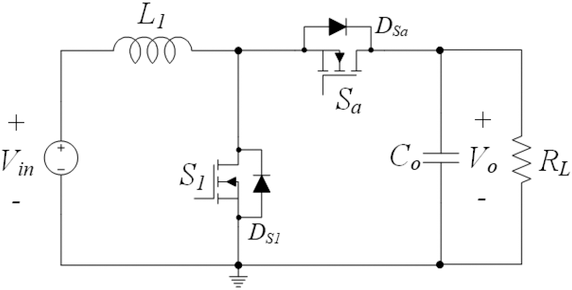
\includegraphics[width=0.5\textwidth]{Images/Implementation/Conventional-synchronous-boost-converter.png}
    \caption{Synchronous boost converter topology \cite{lee_high-efficiency_2019}.}
    \label{fig:sync_boost}
\end{figure}

\subsection{Dimensioning}
Let us first define the design goals of the synchronous boost converter. The converter must be able to step up the voltage from the solar panels, which may consist of a maximum of 40 cells (Maxeon Gen 3 from SunPower) connected in series, a minimum of 20 cells in series, and is optimized for 35 cells (Figure~\ref{tab:pv_conditions}). 
The converter must charge a lithium-ion battery with a nominal voltage of 43.2~V. 
The switching frequency was defined as 100~kHz. This relatively high frequency allows the use of smaller inductors and capacitors, while still avoiding excessive switching losses.

Table~\ref{tab:converter_constraints} and \ref{tab:pv_conditions} summarizes the system requirements.



\begin{table}[!ht]
\centering

\begin{minipage}{0.48\textwidth}
\centering
\captionof{table}{\acs{pv} panel parameters at \acs{mppt}.}
\label{tab:pv_conditions}
\begin{tabular}{lccc}
\hline
Configuration & $V_{mppt}$ (V) & $I_{mppt}$ (A) & $P_{mppt}$ (W) \\
\hline
40 cells & 24.68 & 6.05 & 139.6 \\
35 cells & 21.875 & 6.05 & 122.15 \\
20 cells & 12.34 & 6.05 & 69.8 \\
\hline
\end{tabular}
\end{minipage}
\hfill
\begin{minipage}{0.48\textwidth}
\centering
\captionof{table}{Converter design constraints.}
\label{tab:converter_constraints}
\begin{tabular}{lc}
\hline
Parameter & Value \\
\hline
Battery voltage (nominal) & 43.2 V \\
Battery voltage (max) & 50.4 V \\
Battery voltage (min) & 30 V \\
$\Delta V_o$ & 0.1 V \\
$\Delta V_i$ & 0.5 V \\
$\Delta I_in$ & 0.6 A \\
Efficiency  & $>$ 90\% \\
\hline
\end{tabular}
\end{minipage}

\end{table}

\textcolor{red}{talvez tirar este delta Iin}

Since the load is a battery, the output ripple voltage must be limited to avoid aging and heating. The industry standard is to limit the output voltage ripple to 0.5\% of the nominal voltage. As for  Therefore, the values presented in Table~\ref{tab:converter_constraints} were selected. Also, the voltage output voltage ripple must be low to avoid unexpected behavior of the electronic components that are also connected to the battery. As for the input (the solar panel) the voltage ripple must be low for easier measurement and precise control. As for the current, it must be low to reduce electromagnetic interference and losses.

\subsubsection{Inductor}
The inductor is one of the most important components in the boost converter since it is responsible for storing energy and releasing it to the load. 

The choice of an inductor will highly influence the performance of the converter. High inductance will generate low current ripple, however it generates losses due to its internal resistance. On the other hand a smaller inductance will generate high current ripples, high stress in components and high magnetic interference.

On the other hand, a smaller inductance will generate high current ripples that can cause the system to operate in \ac{dcm}. In \ac{dcm} the inductor current reaches zero during the switching period, which means that the energy stored in the inductor is not enough to supply the load during the off time. This can cause high current and voltage ripples, which can damage the components and reduce the efficiency of the converter. Therefore, it is important to ensure that the inductance is high enough to operate in \ac{ccm}.


The equation that describes the inductor is defined as:
\begin{equation}
    V_L = L \cdot \frac{dI_L}{dt} = L \cdot \frac{\Delta i_l}{\Delta t} \Leftrightarrow L = \frac{V_L \Delta t}{\Delta i_L}
    \label{eq:inductor1}
\end{equation}

In the first stage (transistor in conduction mode), the voltage in the inductor is equal to the input voltage and it occurs for $D \cdot T$ seconds. Therefore, the ripple current in the inductor can be defined as follows:

\begin{equation}
    \Delta I_L = \frac{V_{in} \cdot D \cdot T}{L}
\end{equation}

As for the current ripple, it can be described using the riple factor and the average current in the inductor as follows.
\begin{equation}
    r = \frac{\Delta I_L}{I_{L,avg}}
    \label{eq:riple factor}
\end{equation}

\begin{equation}
    I_{L,avg} = \frac{I_o}{1-D}
    \label{eq:ilavg}
\end{equation}

Using Equation~\ref{eq:ilavg}, \ref{eq:riple factor}, \ref{eq:inductor1} and \ref{eq:duty}, the following equation is achieved:

\begin{equation}
    L = \frac{V_{in} (1-D)DT}{I_o \cdot r} = \frac{V_{out}(1-D)^2DT}{I_o \cdot r}
    \label{eq:L}
\end{equation}

The value of D that maximizes Equation~\ref{eq:L} is 1/3, which results in the critical inductance formula:

\begin{equation}
    MAX[(1-D)^2\cdot D]= (1-1/3)^2 \cdot 1/3= \frac{4}{27}
\end{equation}
\begin{equation}
    L_{critical} = \frac{4}{27} \cdot \frac{V_o}{I_o \cdot r \cdot f}
\end{equation}

Using the maximum battery voltage (50.4~V) and the maximum current ($I_{pv}+Margin=10~A$), and a ripple factor of 2 which is equivalent  to the \ac{ccm} limit we achieve the following result:

\begin{equation}
    L_{critical} = \frac{4}{27} \cdot \frac{50.4}{10 \cdot 2 \cdot 100000} = 3.73 \mu H
\end{equation}

This is a reference value, if it were used it would highly stress the components, generating heat, magnetic interference and high current ripples. Therefore, the calculation was repeated aiming the output current ripple of 0.6~A, which is the value defined in Table~\ref{tab:converter_constraints}. Solving equation~\ref{eq:riple factor} in terms of the output current ripple, the following equation is achieved:
\begin{equation}
    r = \frac{\Delta I_L}{I_{L,avg}} = \frac{\Delta I_{out} \cdot (1-D)}{\frac{I_{out}}{(1-D)}} = \frac{\Delta I_{out} \cdot (1-D)^2}{I_{out}}
\end{equation}


\begin{equation}
    L_{critical} = \frac{4}{27} \cdot \frac{50.4}{10 \cdot 0.4 \cdot 100000} = 18.66 \mu H
\end{equation}

The final value of the inductor was defines as \textcolor{red}{68uH} 100~$\mu H$, which results in a maximum inductor ripple current of 1.26~A and an output current ripple of 0.53~A. \textcolor{red}{refazer o calculo}

To select the apropriate inductor, the rated current and the saturation current must be taken into account. The rated current is the maximum current that the inductor can handle without overheating. In this case the rated current must be higher that the maximum short circuit current of the biggest solar panel configuration (40 cells in series), which is 6.56~A. Some margin must be added to this value, so the rated current must be higher than 10~A.

The saturation current is the maximum current that the inductor can handle without saturating. When the inductor saturates, the inductance drops significantly, which can cause high current ripples and damage the components. Therefore, the saturation current must be:

\begin{equation}
    I_{sat} > I_{in} + \frac{\Delta I_L}{2} = 6.56 + \frac{1.26}{2} = 7.19~A
\end{equation}

The inductor chosen was the 74437529203680 from Würth Elektronik, which has an inductance of 68~$\mu H$, a rated current of 16~A and a saturation current of 7.2~A ($|\Delta L/L|<10\%$) and 10.6~A ($|\Delta L/L|<30\%$). The saturation current is too close with the objective, however since the inductance is higher than what is needed, the inductance would still be acceptable even at -30\% inductance. 

Additionally, it has a low \ac{esr} of only 10.3~$m\Omega$, high self resonant frequency of 5.7~MHz and high Operating voltage of 250~V.

\subsubsection{Capacitor}
    The output capacitor is responsible for smoothing the output voltage and reducing the voltage ripple. The capacitor electric characteristic can be described by the following equation:
    \begin{equation}
        i_c = C \frac{dv_o}{d_t}
    \end{equation}

    Based on this equation, the capacitor value can be calculated based on the desired voltage ripple and the load current as follows:
    \begin{equation}
        i_c = C_o  \frac{\Delta V_o}{\Delta t} = C_o \frac{\Delta V_o}{D \cdot T } \Leftrightarrow C_o = \frac{I_o D}{\Delta V_o \cdot f} = \frac{I_{in} (1-D)D}{\Delta V_o \cdot f}
    \end{equation}

    Using the maximum input current of 10~A, a duty cycle of 0.5 (value that maximizes the formula), a voltage ripple of 0.1~V and a switching frequency of 100~kHz, the following value is achieved:
    \begin{equation}
        C_o = \frac{10 \cdot (1-0.5) \cdot 0.5}{0.1 \cdot 100000} = 250 \mu F
    \end{equation}

    The same can be done for the input capacitor, but in this case the voltage ripple is not as critical as in the output capacitor, since the input voltage is not directly connected to the load. Therefore, a voltage ripple of 0.5~V was used:
    \begin{equation}
        C_{in} = i_{in} \cdot \frac{\Delta t}{\Delta V_i} = \frac{i_{in} \cdot D}{\Delta V_{in} \cdot f}  =  \frac{10 \cdot 0.5}{0.5 \cdot 100000} = 100 \mu F
    \end{equation}

    To choose the appropriate capacitors, the voltage rating, current ripple and \ac{esr} must be taken into account. The voltage rating must be higher than:
    \begin{equation}
        V_{rating} > MAX(V_{in}) + \Delta V_{in} = 28.5 + 0.5 = 29~V
    \end{equation}

    Where 28.5 is the maximum voltage of a solar panel (40 cells in series) and 0.5 is the voltage ripple defined in Table~\ref{tab:converter_constraints}.

    The current ripple must higher than the RMS input current, which can be calculated based on the RMS formula for triangle wave as follows:
    \begin{equation}
        I_{ripple} > \frac{\Delta I / 2}{\sqrt{3}} = \frac{1.26 / 2}{\sqrt{3}} = 0.36~A
    \end{equation}

    As for the \ac{esr} the value must be as low as possible to reduce the power losses. 

    After analyzing the market, the input capacitor selected was the 870575875006 which is a 56~$\mu F$ (2 in parallel) with a voltage rating of 63~V and a ripple current of 2.4~A each (total of 4.8~A). The main reason for this choice was his low \ac{esr} (22~$m\Omega$) compared to other capacitors with similar values. Additionally, by using two capacitors in parallel, the \ac{esr} is reduced even further and the current ripple that they with stand is higher and the reliability of the system is increased.

    The same process was repeated for the output capacitor, but in this case the voltage rating must be higher than the maximum battery voltage, which is 50.4~V. The current ripple must be higher than the RMS output current, which can be calculated as follows:
    \begin{equation}
        V_{rating} > MAX(V_{out}) + \Delta V_{out} = 50.4 + 0.1 = 50.5~V
    \end{equation}
    \begin{equation}
        I_{ripple} > \sqrt{\frac{I_{in}^2}{4} + \frac{\Delta I ^2}{12} \cdot (1-D)^2} = \sqrt{\frac{6.56^2}{4} + \frac{1.28 ^2}{12} \cdot (1-0.27)^2} = 3.29~A
    \end{equation}

    The ripple current in the output capacitor is much higher than in the input capacitor, and it is not a common value for electrolytic capacitor, therefore instead of using a single capacitor, multiple capacitors in parallel will be used to achieve the desired current ripple rating.

    After simulations and analyzing the market, the output capacitor value were increased due to the output current ripple dependency on the output voltage ripple. The final capacitor chosen was the 860040875005 with 100~$\mu F$  (5 in parallel, so 5x100~$\mu F$) with a voltage rating of 100V and a ripple current of 0.8~A each (total of 4~A). Some other options were considered, and compared for optimization in section~\ref{subsubsect:Sim_Boost}. 

    Additionally, the output and input needs to filtered to reduce the high frequency noise generated by the switching. This is achieved by adding a small capacitor in parallel with the main capacitors. The values use are 1~$\mu F$ and 0.1~$\mu F$. For this use case ceramic capacitors are better since their stacked multilayer construction provides extremely low \ac{esr} and \ac{esl} which over all let them maintain low impedance up into the MHz range.

\subsubsection{Transistor and gate driver}
    The transistor is the switching device on a synchronous boost converter. The choice of the transistor will highly influence the behavior and performance of the converter.

    When selecting a transistor for a switching converter, not only the maximum rating mater but the switching speed and internal resistance are also quite important. 
    
    There are many types of transistors (IGBT, MOSFET,  GaN, etc.), however, at this frequency (100~kHz) and power level the choice is between MOSFETs and GaN transistors (Figure~\ref{fig:tech_transistor}). The GaN (Gallium Nitride) transistor technologies has appeared in 1993 in lab experiments, however it has only reached the market more recently, first for radio frequency products in 2004 and only in 2009 for power electronics. The advantage of GaN transistors is their low internal resistance and very fast switching speed, which can significantly reduce the switching losses and therefore increasing the efficiency of the converter. Additionally, they have a high energy density and lower Vgs(on). However, they are more expensive and require a precise gate driver to operate correctly because there max(Vgs) is usually low. 

    In applications where the efficiency is a key factor in the design like solar inverters or \ac{mppt}, it is better to use the component that has lower Internal (On) Resistance (RdsOn) and supports higher switching frequency. In this case, GaN would be a better fit. MOSFET or Silicon Carbide MOSFET would take the second place since MOSFETs can handle higher switching frequencies as compared to IGBTs \cite{talat2024igbt}.

    There are a lot of options in the market, however there was one in specifically that standout due to their compact size, while having integrated gate driver and two transistors in the same package. The \ac{ic} is the EPC23102, which was designed for power applications, with an incredibly low RdsOn (only 5.2~$m\Omega$), 35~A of maximum power and a maximum operating voltage of 100~V.
    
    Additionally, it has incorporates shoot-through protection that protects the transistor from a control error, however a dead time needs to be introduced in software. It uses a DFN package which is good for heat dissipation and can always be attached to a heat sink for better performance. 


    \begin{figure}[!ht]
        \centering
        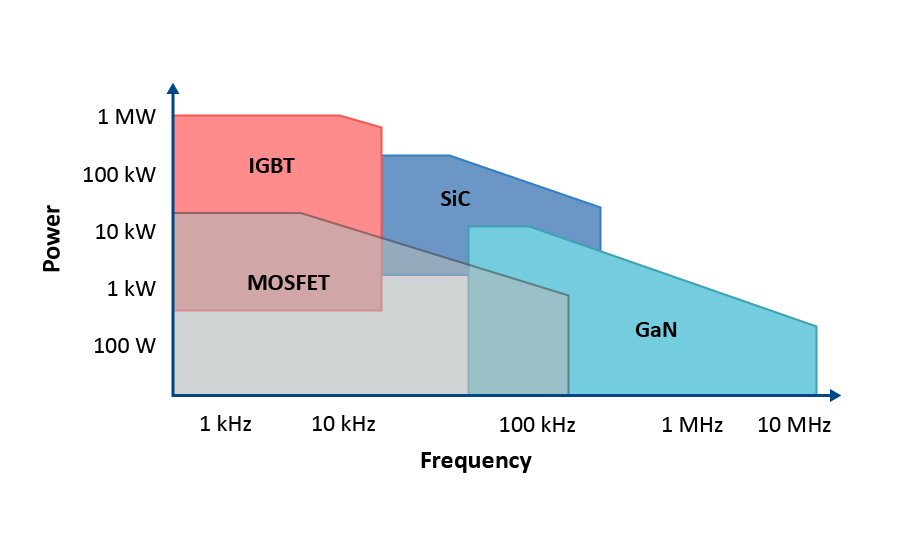
\includegraphics[width=0.7\textwidth]{Images/Implementation/tescnologies.jpg}
        \caption{Technologies selection based on power and switching frequency \cite{talat2024igbt}.}
        \label{fig:tech_transistor}
    \end{figure}

    \subsection{Simulations}
        \textcolor{red}{Objective}

        \subsubsection{Solar Panel model}

            The simulations started at LTspice with the aim to test the converter at different conditions. To achieve that, a \ac{pv} electrical model of the cells were designed using a five parameter model (1M5P) configuration. There are more electrical models that can simulate a solar panel, some with more accuracy but more complex. This model was perfect for the aim of the simulation since it is both reliable and simple.

            The 1M5P model represents the solar cell through a single diode equivalent circuit composed of a current source in parallel with one diode, a series resistance $R_s$, and a shunt (parallel) resistance $R_{sh}$, as shown in Figure~\ref{fig:pv_model}. The current source represents the photogenerated current $I_{ph}$, which is proportional to the incident irradiance, while the diode accounts for the non linear $I$-$V$ characteristic of the p-n junction. The series resistance models the losses associated with the material bulk resistance, metal contacts and interconnections, whereas the shunt resistance represents the leakage currents through the cell, typically caused by manufacturing defects.

            The output current of the model is given by the characteristic equation~\ref{eq:1m5p}, where $I_0$ is the diode saturation current, $n$ is the diode ideality factor, and $V_t$ is the thermal voltage \cite{LOBRANO2013894}. Together with $I_{ph}$, $R_s$ and $R_{sh}$, these constitute the five parameters that give the model its name.

            \begin{equation}
                I = I_{ph} - I_0 \left[ \exp\left(\frac{V + I R_s}{n V_t}\right) - 1 \right] - \frac{V + I R_s}{R_{sh}}
                \label{eq:1m5p}
            \end{equation}

            These parameters are not directly provided by manufacturers, but can be extracted from the standard datasheet values, namely the open-circuit voltage ($V_{oc}$), short-circuit current ($I_{sc}$), voltage and current at the \ac{mpp} ($V_{mp}$, $I_{mp}$), and the respective temperature coefficients, through a set of equations that ensure the model matches these reference points under Standard Test Conditions (STC). There are several ways to do it, however it is outside the range of this work. To simplify, calculations were carried using online tools and will not be explained in detailed here. 
            \textcolor{red}{se achar necessario posso escrever as equações aqui}

            This approach allows the panel behavior to be accurately reproduced under different irradiance and temperature conditions, while keeping the circuit implementation simple enough to be integrated directly into LTspice.

            \begin{figure}[!ht]
                \centering
                
\includegraphics[width=0.9\textwidth]{Images/Implementation/PV model.png}
                \caption{Solar panel model diagram (1M5P configuration).}
                \label{fig:pv_model}
            \end{figure}
        
        \subsubsection{Boost Converter}
        \label{subsubsect:Sim_Boost}
            To validate the theoretical  calculations, simulations in LTspice were carried using the boost converter in steady state mode and a fix duty cycle. 

            Considering a solar panel with 35 cells, five points of CC-CV charging curve were chosen to test the performance of the converter. These five points are represented in Figure~\ref{fig:cc-cv points}.
            
            \begin{figure}[!ht]
                \centering
                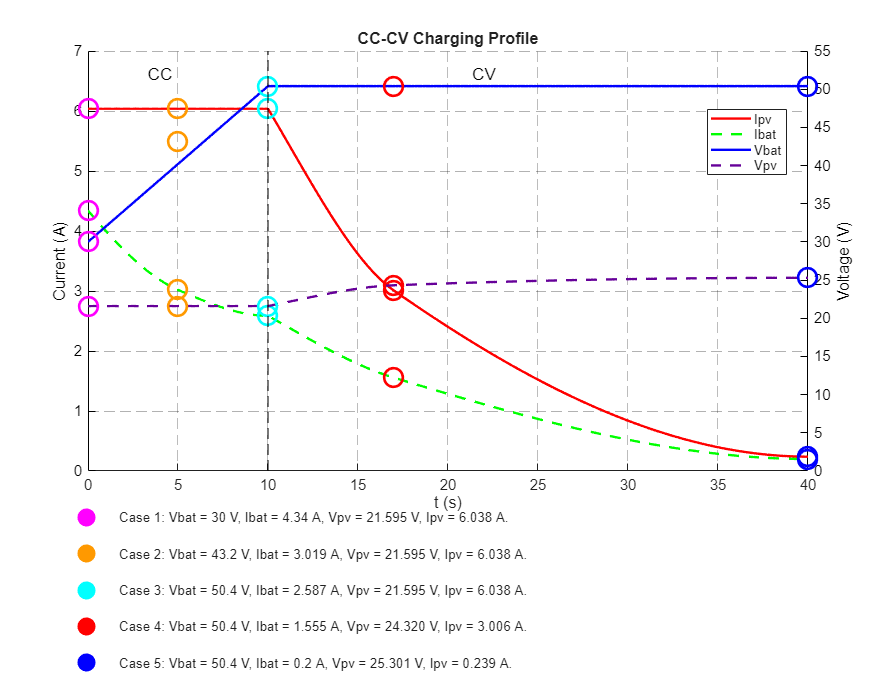
\includegraphics[width=0.9\textwidth]{Images/Implementation/cc_cv_points.png}
                \caption{CC-CV charge characteristics and analysis point selection.}
                \label{fig:cc-cv points}
            \end{figure}

            It is important to note that in this CC-CV curve the constant current is given by the solar panel and not by the battery as it is usually expected. This is only truth due to the maximum charge current of the battery being lower than the current that can be provided by the solar panel. So at CC, the converter is working at \ac{mpp}.

            With this five points chosen, some simulations were carried using capacitors and inductors that would fit the requirements calculated earlier. The objective of these simulations is to optimize the performance of the converter, leading to better choices.

            The model was built in LTspice with approximated models given by the manufactures for higher precision. Only the solar panel model was designed by hand, as previously mentioned.

            The battery was simulated using a voltage source and a resistor representing the internal resistance of the battery.

            The dead time of the transistors was implemented too. Using laboratory measurements, the rising and falling timing was measured and used in simulation. Has for the dead time, it is used the same as in the final prototype.

             \begin{figure}[!ht]
                \centering
                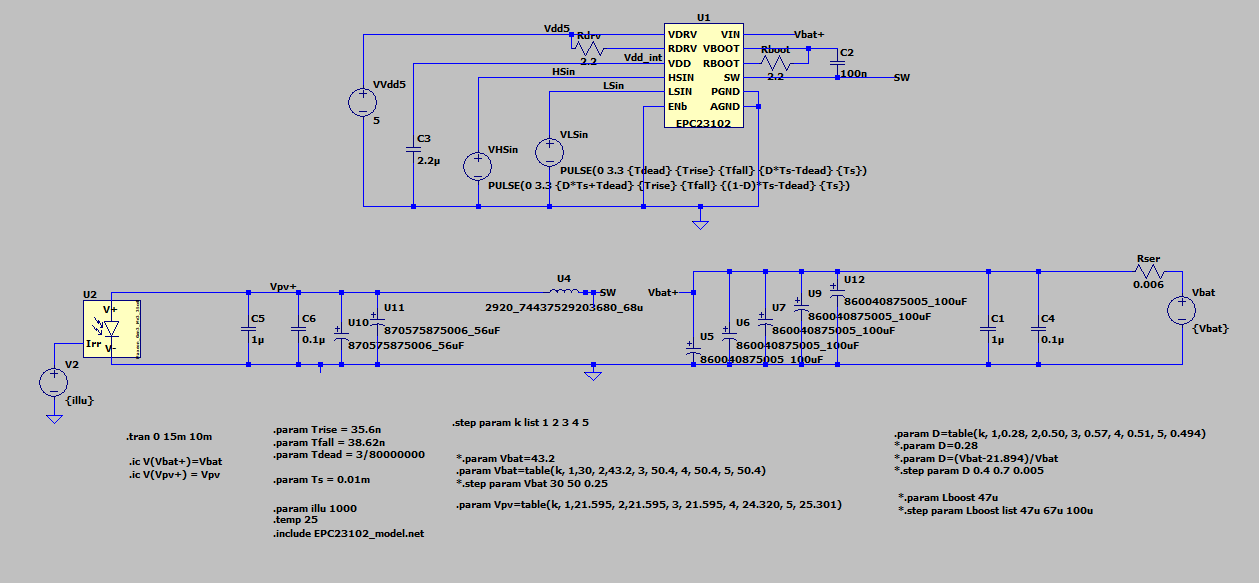
\includegraphics[width=0.9\textwidth]{Images/Implementation/Sim_circuit.png}
                \caption{Simulation circuit schematic.}
                \label{}
            \end{figure}


            The first simulations were carried to choose the input and output capacitors. The idea is to simulate the circuit using a known inductor (68~uH) and change the capacitors for different configurations. All configurations are overdimensioned to give low ripples (current and voltage). So the main factor is the efficiency of the converter.

            In Table~\ref{tab:loss_capacitors_2} is shown the results. The efficiency of all combinations are very high however the highest is the one with two 56~uF as input capacitors and tree 220~uF capacitors as output capacitors. Unfortunately the 220~uF were not available at the moment, so the second best option was chosen, the five 100~uF capacitors.

            It is worth noting that this is a simulation and therefore the efficiency is higher than what will be measured in laboratory results. Additionally, the difference between each combination it is very small. To make the product cheaper the third option would be as great as the one chosen.

            
            \begin{table}[!ht]
                \caption{Loss (\%) for different capacitor configurations (Cin, Cout).}
                \centering
                \begin{tabular}{|c|cccc|}
                \hline
                \textbf{Case \#} & \textbf{2x56 $\mu$F, 3x220 $\mu$F} & \textbf{100 $\mu$F, 3x220 $\mu$F} & \textbf{100 $\mu$F, 5x100 $\mu$F} & \textbf{2x56 $\mu$F, 5x100 $\mu$F} \\
                \hline
                1 & 0.5729 & 0.5796 & 0.5856 & 0.5788 \\
                2 & 0.6762 & 0.6985 & 0.7069 & 0.6844 \\
                3 & 0.7359 & 0.7655 & 0.7743 & 0.7449 \\
                4 & 0.6654 & 0.7091 & 0.7161 & 0.6735 \\
                5 & 3.4177 & 3.7148 & 3.7554 & 3.4671 \\
                \hline
                \end{tabular}
                
                \label{tab:loss_capacitors_2}
            \end{table}

            Similar to the previous simulation, the inductor was chosen by keeping all components with the same values (the capacitors used were Cin = 2x56uF and Cout = 5x100uF) and changing the inductor. Similar to before, all inductors simulated are within the minimum required.

            The losses for each case are represented in Table~\ref{tab:loss_inductance_2}. Similar to before, the efficiency difference is very low but not as linear as in the previous simulation, likely due to the inductor models chosen.

            The inductor chosen will highly influence the input ripple which can generate heat, and electrical interference. Table~\ref{tab:delta_iin_inductance} shows the different ripple currents for each inductor in each case of the CC-CV curve. The 22~uF inductor showed higher ripple current reaching values close to the input current. The inductor chosen was the 68~uF since it has overall good efficiency and reasonable input current ripple.


            \begin{table}[!ht]
                \caption{Loss (\%) for different inductance values.}
                \centering
                \begin{tabular}{|c|ccccc|}
                \hline
                \textbf{Case \#} & \textbf{22 $\mu$H} & \textbf{33 $\mu$H} & \textbf{47 $\mu$H} & \textbf{68 $\mu$H} & \textbf{100 $\mu$H} \\
                \hline
                1 & 0.4206 & 0.4439 & 0.5453 & 0.5788 & 1.2659 \\
                2 & 0.6645 & 0.6793 & 0.6627 & 0.6844 & 1.3664 \\
                3 & 0.7883 & 0.8076 & 0.7290 & 0.7449 & 1.4193 \\
                4 & 1.0556 & 1.0583 & 0.6867 & 0.6735 & 0.9624 \\
                5 & 6.7045 & 6.6230 & 3.6556 & 3.4671 & 3.8177 \\
                \hline
                \end{tabular}
                \label{tab:loss_inductance_2}
            \end{table}


            \begin{table}[!ht]
                \caption{$\Delta i_{in}$ ($I_{in,\max} - I_{in,\min}$) for different inductance values.}
                \centering
                \begin{tabular}{|c|ccccc|}
                \hline
                \textbf{Case \#} & \textbf{22 $\mu$H} & \textbf{33 $\mu$H} & \textbf{47 $\mu$H} & \textbf{68 $\mu$H} & \textbf{100 $\mu$H} \\
                \hline
                1 & 2.6939 & 1.8906 & 1.3256 & 0.9781 & 0.6251 \\
                2 & 4.7934 & 3.3416 & 2.3354 & 1.7066 & 1.0707 \\
                3 & 5.4733 & 3.8253 & 2.6813 & 1.9644 & 1.2839 \\
                4 & 5.5596 & 3.8565 & 2.7075 & 2.0139 & 1.2925 \\
                5 & 5.5520 & 3.8510 & 2.6903 & 1.9636 & 1.2344 \\
                \hline
                \end{tabular}
                \label{tab:delta_iin_inductance}
            \end{table}

           Now that the converter components are all chosen, the following measurements were taken in LTspice:

            \begin{table}[!ht]
            \centering
            \caption{Ripple and Power Loss Summary for Each Operating Step}
            \label{tab:ripple_loss}
            \begin{tabular}{|c|cccc|}
            \hline
            \textbf{Case \#} & \textbf{$\Delta V_{bat}$ (V)} & \textbf{$\Delta V_{pv}$ (V)} & \textbf{$\Delta I_{in}$ (A)} & \textbf{Loss (\%)} \\
            \hline
            1 & 0.0406 & 0.0145 & 0.9781 & 0.578 \\
            2 & 0.0491 & 0.0212 & 1.7066 & 0.684 \\
            3 & 0.0529 & 0.0244 & 1.9644 & 0.745 \\
            4 & 0.0406 & 0.0220 & 2.0139 & 0.674 \\
            5 & 0.0302 & 0.0215 & 1.9636 & 3.464 \\
            \hline
            \end{tabular}
            \end{table}

            Both voltage ripples are lower than what was defined as the goal in Table~\ref{tab:converter_constraints}. As for the current ripple it is still reasonable. The losses/efficiency are also higher than what was aimed, reaching values up to 99.4\%, in simulation. 

           A voltage sweep were performed, and as expected the efficiency drop with the increase of output voltage (Figure~\ref{fig:voltage_sweep}). Also, as mentioned earlier, the output current drop because in \ac{cc} mode the solar panel current is constant, so the output current drops with the increase of battery voltage due to the power conservation principle.

            \begin{figure}[!ht]
                \centering
                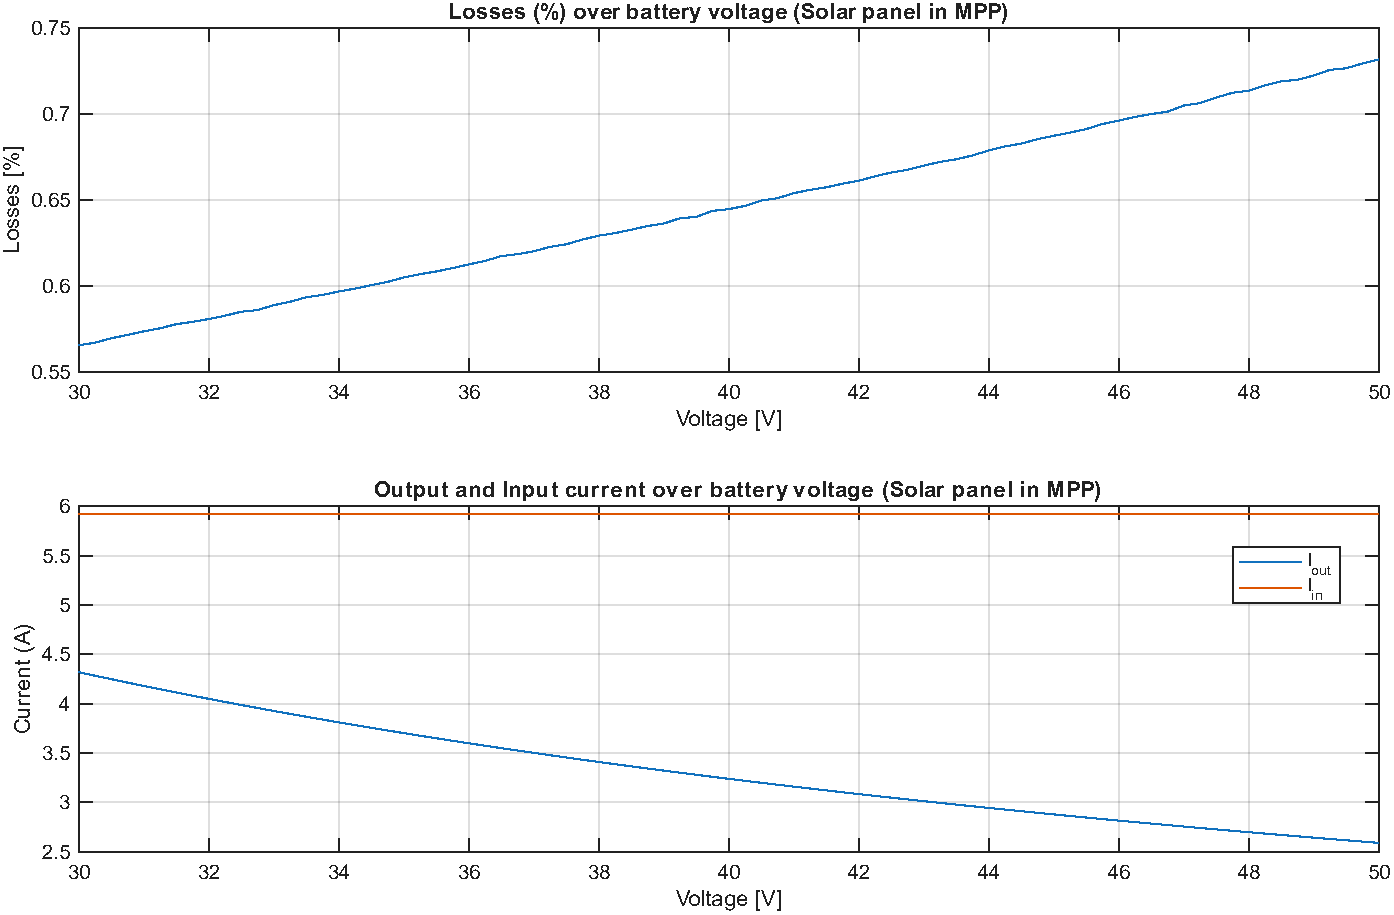
\includegraphics[width=0.7\textwidth]{Images/Implementation/vbat__sweep_sim_res.pdf}
                \caption{Battery voltage sweep simulation results.}
                \label{fig:voltage_sweep}
            \end{figure}

            Note: in Section~\ref{subsec:PCB_design_MPPT} it is mention the addition of two shotcky diodes that were not considered in simulations. These diodes slightly increase the efficiency of the converter (+0.03\%) due to their lower forward voltage.

            \textcolor{red}{Add wave forms??!?!?!}

    \subsection{Power Loss Estimation}
        \label{subsubsec:loss_estimation}

        Although LTspice provides an accurate estimation of the converter efficiency, it does not directly identify the contribution of each component to the total power dissipation. Therefore, an analytical power loss model was developed in MATLAB to estimate the individual losses of each component of the proposed synchronous boost converter. The model uses the electrical parameters of the selected components obtained from their datasheets together with the converter operating conditions.

        The total converter losses are obtained by summing the losses associated with the GaN transistors, inductor, capacitors, dead time and gate driver,

        \begin{equation}
        P_{loss}=P_{cond_{HS}}+P_{cond_{LS}}+P_{sw_{HS}}+P_{sw_{LS}}+P_{L}+P_{C}+P_{dead}+P_{gate}.
        \end{equation}

        The converter efficiency is then calculated as

        \begin{equation}
        \eta=\frac{P_{out}}{P_{out}+P_{loss}}\times100\%.
        \end{equation}

        The conduction losses of each GaN transistor are given by

        \begin{equation}
        P_{cond}=I_{RMS}^{2}R_{DS(on)}.
        \end{equation}

        These losses are primarily caused by the on state resistance of the transistors, resulting in power dissipation whenever current flows through the channel. 

        The switching losses are estimated using Equation~\ref{eq:psw}, 
        which takes into account the loses during the period when the transistor is not fully nor fully off. Also, the losses associated with charging and discharging the output capacitance of each transistor.

        \begin{equation}
        P_{sw}=\frac{1}{2}V_{out}I_{L_{AVG}}(t_r+t_f)f_{sw} + \frac{1}{2}C_{oss}V_{out}^{2}f_{sw}
        \label{eq:psw}
        \end{equation}

        The dead-time losses are calculated using Equation~\ref{eq:pdead}. These losses originate from the conduction of the reverse conduction path during the dead-time interval required to prevent shoot through. This reverse condition path is either from the third quadrant conduction from the GaN device or from the parallel schottky diode added later in version 1.1 (this is explained in Section \textcolor{red}{?})

        \begin{equation}
        P_{dead}=2\cdot  V_f \cdot I_{L_{AVG}} \cdot t_{dead} \cdot f_{sw}.
        \label{eq:pdead}
        \end{equation}



        The inductor and capacitor losses are estimated using the RMS current passing through them and their \ac{esr}

        \begin{equation}
        P_L=I_{L_{RMS}}^{2}ESR.
        \end{equation}

        \begin{equation}
        P_C=I_{C_{RMS}}^{2}ESR,
        \end{equation}

        Although magnetic core losses of the inductor could be estimated too, the selected manufacturer does not provide the required magnetic material parameters. Consequently, only the winding copper losses are considered, leading to a slight underestimation of the total converter losses.

        Finally, the gate driver losses are estimated using Equation~\ref{eq:gate_drive} which takes into account the energy needed to drive the transistors. Although the EPC23102 has an internal gate driver, this is still relevant.

        \begin{equation}
        P_{gate}= (Qg_{LS} + Qg_{HS})* Vdrv * fsw.
        \label{eq:gate_drive}
        \end{equation}

        Figure~\ref{fig:loss_breakdown} presents the resulting power loss distribution. The calculated total power loss is approximately 1.188~W, corresponding to an efficiency of 99.10\%, which agrees well with the LTspice simulation results presented in the previous section.

        \begin{figure}[!ht]
            \centering
            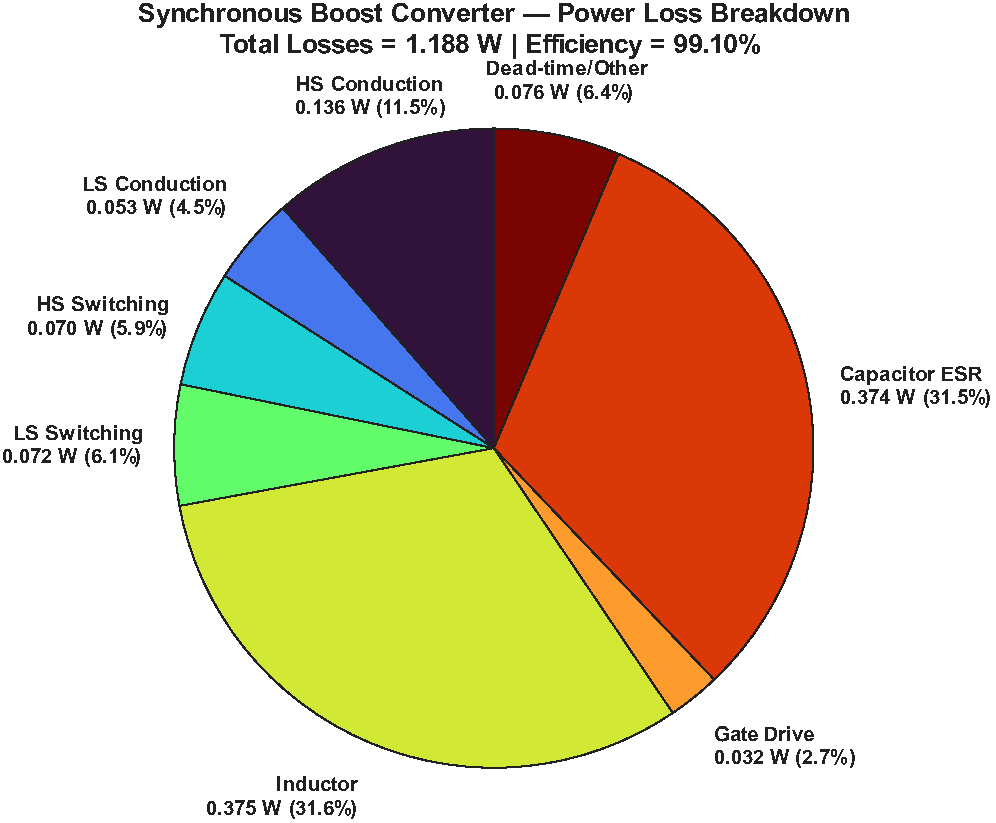
\includegraphics[width=0.6\textwidth]{Images/Implementation/Losses.pdf}
            \caption{Analytical power loss distribution of the synchronous boost converter for Case~1.}
            \label{fig:loss_breakdown}
        \end{figure}

        The largest contributors to the total losses are the inductor copper losses and the capacitor ESR losses, each accounting for approximately 31.5\% of the total power dissipation. This highlights the importance of selecting an inductor with low winding resistance and capacitors with low ESR, as these passive components dominate the converter losses.

        The conduction losses of the GaN transistors account for approximately 16\% of the total losses, showing the importance of choosing transistors with low conduction resistance. The high-side device dissipating more power than the low-side transistor due to its longer conduction interval. Switching losses represent approximately 12\% of the total losses, including both transition losses and the energy required to charge and discharge the output capacitances. Dead-time losses contribute approximately 7\%, while the gate driver losses are almost negligible (only 2.7\%).

        Additionally, all \ac{pcb} connections have an inductance that will represent losses too. 

        Overall, the analysis indicates that nearly two-thirds of the converter losses originate from the passive components, whereas the semiconductor devices account for approximately one-third. It should be noted that the presented values are based on analytical equations and datasheet parameters. Since magnetic core losses were not considered, the calculated efficiency represents a slight overestimation of the actual converter performance.

        However, both simulation and theoretical analysis indicate that the choice of each components lead to a highly efficient converter.



\clearpage
\section{Processing unit}

    \textcolor{red}{Maybe i will remove this part \{}
    Several types of processing units can be considered for this project, including \acp{mcu}, \acp{fpga}, and \acp{asic}.  

    \acp{asic} are custom-designed integrated circuits optimized for specific applications, offering high efficiency and performance. However, they are typically expensive and time-consuming to design and manufacture. Although commercially available \acp{asic}, commonly referred to as \acp{ic}, mitigate these drawbacks, they are usually made for a specific application and therefore not suitable for the high performance and flexibility required in this project, as discussed in Section~\ref{sec:ICs}.  

        \acp{fpga} are reconfigurable devices capable of implementing custom digital circuits through programmable logic blocks based on look-up tables (LUTs) and interconnections~\cite{231340}. Their main advantage lies in their inherent parallel processing capability, which enables high-performance operation. Nevertheless, \acp{fpga} generally present high costs, high design complexity, and volatile configuration memory, requiring reprogramming after power loss~\cite{ampheo_fpga_vs_microcontroller_2025,FPGA_Implementation_MPPT}.  

        In contrast, \acp{mcu} are widely adopted in embedded systems due to their low cost, ease of use, and versatility. They integrate processing, memory, and peripherals in a single non-volatile device, simplifying hardware design and development. Although their sequential execution limits parallel processing performance compared to \acp{fpga}, modern \acp{mcu} provide sufficient computational capability for many control and signal-processing tasks~\cite{ampheo_fpga_vs_microcontroller_2025}.  

        Considering the emphasis on low cost, reduced development time, and implementation simplicity, a \ac{mcu} is selected for this application. Furthermore, the performance of current \acp{mcu} is adequate to meet the requirements of the \ac{mppt} algorithm and the battery charging strategy.

        \textcolor{red}{------------\}}

        A \acf{mcu} typically consists of three fundamental components: a central processing unit (CPU), memory, and peripheral modules. The CPU executes program instructions and performs arithmetic and logical operations. Memory is generally divided into non-volatile memory (Flash) for program storage and volatile memory (SRAM) for data and runtime variables. Peripheral modules provide interfaces to the external environment and may include analog-to-digital converters (ADCs), timers, pulse-width modulation (PWM) units, communication interfaces (such as UART, SPI, I²C and \acs{can}), and general-purpose input/output (GPIO) ports. The integration of these components enables standalone operation without the need for extensive external circuitry~\cite{ibm_microcontroller_2025}.

         When selecting a \acs{mcu} for a specific application, the first factor to consider is to use an 8, 16, or 32 bit \acs{mcu}. For this application, a 16-bit \acs{mcu} would probably be sufficient, however to ensure future-proof and compatibility with other \ac{tsb} systems, the choice is for a 32-bit \ac{mcu}. Besides, nowadays, 32-bit \acp{mcu} are considered the industry standard since most embedded system \ac{red} effort is focused on 32-bit cores, and thus both architectures can achieve similar power consumption~\cite{embedded_upgrading_mcu_designs_2025}.
          There are two main architectures for 32-bit \acp{mcu}: AVR and ARM. Being ARM, the most widely used architecture in the industry and the most advanced, it was chosen for this project~\cite{ampheo_fpga_vs_microcontroller_2025}. 

        STM32 family of \acp{mcu} offers a wide range of solutions with different characteristics, making it suitable for various applications, including this project. This family of microcontrolers is used by \ac{tsb}, so it will be used for this project to maintain the standard. 

        The \ac{mcu} requirements for this project are:
        \begin{itemize}[leftmargin=4em, itemsep=1pt, topsep=2pt]
            \item Fast clock frequency: 80~MHz or higher;
            \item Support 1x CAN peripheral, 1x I2C, 1x UART;
            \item Able to read 4 or more analog signals;
            \item 12bit ADC or more.
        \end{itemize}

        The final decision was the STM32L476. Although it is not the most suitable STM32 microcontroller for this application, it was selected due to its low cost and because it was already widely used within \ac{tsb}, reducing development time and associated risks.

        The STM32L476 is based on an ARM Cortex-M4 core with floating-point support and operates at frequencies up to 80~MHz. The device provides 1~MB of Flash memory and 128~kB of SRAM, which is more than sufficient for the implementation of the \ac{mppt} algorithm, data acquisition, communication protocols, and debugging features. Regarding peripherals, it includes three 12-bit ADCs with up to 16 external channels each, multiple general-purpose and advanced timers capable of high-resolution PWM generation, several communication interfaces (CAN, SPI, I\textsuperscript{2}C, UART, USB), and DMA controllers that allow peripheral operation with minimal CPU intervention.

        These features make the STM32L476 particularly attractive for power electronics applications, where simultaneous voltage and current measurements, fast PWM generation, and real-time control execution are required. Furthermore, the presence of a hardware floating-point unit simplifies the implementation of control algorithms and numerical calculations.

        If there were no limitations, a microcontroller with a higher clock frequency would have been selected, increasing both the PWM duty-cycle resolution and the available computational power. Additionally, a device with native 16-bit ADCs would improve measurement accuracy and reduce quantization effects. Nevertheless, the STM32L476 provides sufficient performance and peripheral resources to meet the requirements of this application.


\section{Sensors} 

\subsection{Voltage and current sensing}
    Accurate voltage and current measurements are essential for MPPT operation, since tracking algorithms directly rely on these quantities to estimate power and adjust the operating point of the \ac{pv} array. Measurement noise or inaccuracies directly impact tracking efficiency, especially in high frequency switching DC-DC converters.

    Voltage sensing is generally straightforward and can be implemented using resistive voltage dividers followed by ADC. Additionally, it is suggested to use an op-amp as a buffer to reduce the impact of the ADC input capacitor, while charging. This buffer reduces noise and improves the accuracy of the measurement while also allowing the use of higher sampling rates.
    
    Current sensing, however, is more critical and requires careful consideration of the available measurement techniques.

    The two main techniques are:
    \begin{itemize}[leftmargin=4em, itemsep=1pt, topsep=2pt]
        \item Hall effect current sensor.
        \item Shunt resistor sensing with operational amplifiers;
    \end{itemize}

    The hall effect current sensor is a non-invasive method that uses the Hall effect to measure current. It provides galvanic isolation and can do bidirectional measurements. However, it is typically more expensive, has lower bandwidth, and may introduce additional noise due to its magnetic sensing nature.

    As for the shunt resistor sensing, it is a simple and cost-effective method that uses a low-value resistor to convert the current into a voltage drop. This voltage is then amplified using operational amplifiers to match the ADC input range. This method provides high accuracy, low cost, and fast response time, but it requires careful design to minimize power loss since it will dissipate power proportional to the current.

    In the end product a \ac{ic} based on a shunt resistor sensing method was used, which as a built-in amplifier. The sensor chosen was the INA253A2IPWR, which has a PWM rejection block and small form factor that will be extremely useful for this application. However, this \ac{ic} is more expensive than a simple shunt resistor and op-amp solution, but it is more accurate and has a better noise rejection. In the future it can be swapped for a lower cost solution, if the performance is acceptable.

    Both sensors use the internal ADC from the STM32L476, which has a 12 bit ADC (with 3.0V as the reference). The current sensor output an analog voltage that is equal to the current multiplied by 0.2~V/A. Which means that the resolution of the current measured is 3.0/(4096 * 0.2) = 3.66~mA. As for the voltage sensor, it outputs an analog voltage that is equal to the voltage multiplied by 10/210. The resolution is 21 * 3.0/(4096) = 15.38~mV, which is more than enough for this application.

    Both circuits are represented in Appendix~\ref{}. \textcolor{red}{place the apendix reference }

\subsection{Temperature and Irradiance sensors}
    For security reasons it is important to monitor the temperature of the \ac{pcb}. Also, the temperature and irradiance of the \ac{pv} panel are important to monitor for performance analysis and defect detection. Also, this measurements can be used to improve the \ac{mppt} algorithm, since the maximum power point is dependent on temperature and irradiance.

    For temperature sensisng there is a wide range of options, from simple thermistors to more complex digital temperature sensors. For this application a simple thermistor was used, since it is cheap and easy to implement. The thermistor is connected to a voltage divider and the voltage is read by the ADC. The thermistor used to measure ambient temperature and transistor temperature was the ERT-J1VS104FA, which has a resistance of 100k$\Omega$ at 25°C and a B value of 4330K. As for the thermistor used to measure the \ac{pv} panel temperature, it was the 104JT-025, which has a resistance of 100k$\Omega$ at 25°C and a B value of 4390K. 
    The temperature can be calculated using the Steinhart-Hart equation \cite{arduinodiy2015ntc}.

    \begin{equation}
        \frac{1}{T} = A + B \cdot ln(R) + C \cdot ln(R)^3
    \end{equation}

    This equation uses 3 parameters (A, B and C) that are usaly not provided in data sheet but can be calculated using 3 measurements of temperature and resistance. However, the most common approach is to use a simplified version of the equation, which uses only 2 parameters (B and R0). The temperature can be calculated using the following equation:

    \begin{equation}
        \frac{1}{T} = \frac{1}{T_0} + \frac{1}{B} \cdot ln(\frac{R}{R_0})
    \end{equation}

    As for the irradiance sensor, the TSL2591 was used, which is a digital light sensor with a wide dynamic range and high sensitivity. It can measure light intensity from 0.000118 lux to 88,000 lux, making it suitable for various lighting conditions. The sensor communicates with the \ac{mcu} via the I2C protocol, allowing for easy integration and data acquisition.

    Since it measures the light intensity in lux, it is not a direct measurement of irradiance and it needs to be calibrated to convert the lux value to irradiance in W/m\^2. This calibration was done using a irradiance sensor from \textcolor{red}{???} which measures the irradiance in W/m\^2. The calibration was done by measuring the lux and irradiance at the same time and calculating the conversion factor. The conversion factor was found to be \textcolor{red}{????} W/m\^2 per lux at laboratory conditions. This factor changes with the spectral distribution of the light source, so it would need be calibrated for different light sources. 

    There are bether options for irradiance sensors, but this sensor was chosen due to its low cost and easy integration with the \ac{mcu}. The main disadvantage of this sensor is that it is not a direct measurement of irradiance and it needs to be calibrated. However, for laboratory testes it is sufficient since the objective is to record when does the irradiance change to analyze the performance of the \ac{mppt} algorithm. For precise measurements of irradiance, the sensor used to calibrate the TSL2591 can be used, which is a more expensive sensor that provides direct measurements of irradiance but does not provide communication protocol to record the data.

    In the future, if the irradiance value is needed to be used in the \ac{mppt} algorithm, a more precise irradiance sensor is needed. The most precise sensors use a \ac{pv} cell, which based on his temperature, short circuit current and open circuit voltage can provide a good estimation of the irradiance. My suggestion is to design this circuit and use the same cell that is used in the \ac{pv} panel to measure the irradiance. This way, the irradiance measurement will be accurate and with exactly the same spectral distribution as the \ac{pv} panel which will increase the performance of the \ac{mppt} algorithm. This was not implemented in this project due to time constraints, but it is a good option for future work.


\section{Software}
    \subsection{MPPT algorithm}
        \textcolor{red}{simulação em Matlab..}
    \subsection{Firmware}
        \textcolor{red}{Tool de STM32 usada, flow chart, }
    \subsection{Graphical User Interface}
        \textcolor{red}{Funcionalidade, protocoolo de comunicação, como  foi feita, etc.}


\section{Precharge Circuit}
    The precharge circuit is used to safely energize high-capacitance loads by limiting inrush currents during system startup. This section introduces the problem of inrush currents, discusses the adopted mitigation strategy, and presents the final circuit implementation.
    
    \subsection{Problem}

        In the automotive sector, high-capacitance loads such as inverters, motor controllers, and DC/DC converters are commonly encountered. When these systems are connected to a power source, their large input capacitance can lead to significant inrush currents during the transient period. These currents, which can reach the order of kiloamperes, may generate electrical arcing, stress or damage the contactors, and in severe cases cause contact welding, preventing proper disconnection of the circuit. Additionally, such high transient currents can also stress or damage the load itself, particularly sensitive power electronics at the input stage, potentially leading to component failure or reduced operational lifetime.

        In the context of the \ac{mppt}, the battery is connected and disconnected through a relay depending on the system operating conditions, such as the battery state of charge. When the relay closes, the input capacitors of the \ac{mppt} act as an initially uncharged capacitive load, resulting in a high transient current as they are charged from the battery.

        As an example, consider the battery operating at its maximum voltage ($V_{bat} = 50.4~V$) connected to a single \ac{mppt} with an input capacitance of 500~$\mu$F. Initially, the capacitors are fully discharged ($V_c = 0~V$). The total series resistance of the circuit is composed of the internal battery resistance ($R_{bat} = 6~m\Omega$), the equivalent capacitor resistance, and the resistance of the connection cables.

        The cable resistance can vary depending on length and cross-section, but it is typically small and is therefore neglected in this analysis. The equivalent resistance of the capacitors is given by the resistance of a single capacitor ($R_{cap} = 200~m\Omega$) divided by the number of capacitors in parallel ($n = 5$), resulting in:

        \begin{equation}
        R_{caps} = \frac{200~m\Omega}{5} = 40~m\Omega
        \end{equation}

        The total circuit resistance is therefore:

        \begin{equation}
        R_{total} = R_{bat} + R_{caps} + R_{cables} \approx 46~m\Omega
        \end{equation}

        The current flowing into the capacitors at any time can be described by:

        \begin{equation}
        i(t) = \frac{V_s - V_c(t)}{R}
        \label{eq:current_cap}
        \end{equation}

        From this, the worst-case inrush current occurs at $t = 0$, when $V_c = 0$:

        \begin{equation}
        i(0) = \frac{50.4}{0.046} = 1097~A
        \end{equation}

        Such current levels can severely degrade or destroy the contactors over time. Even if immediate failure does not occur, the repeated exposure significantly reduces their operational lifetime.

        This issue becomes even more critical when multiple \acp{mppt} are connected in parallel. In the \ac{sg01} system, four \acp{mppt} are used, resulting in a total capacitance of 2000~$\mu$F and a reduced equivalent resistance of approximately 16~m$\Omega$. In this case, the inrush current increases to approximately 3150~A, further emphasizing the necessity of a precharge strategy.

    \subsection{Solution}

        A common approach to mitigate inrush current in capacitive loads is to introduce a controlled precharge phase, in which the load is temporarily connected to the power source through a series resistance. This resistance limits the initial charging current, allowing the capacitors to charge gradually. Once the voltage across the load reaches a predefined threshold, the resistor is bypassed and the system transitions to normal operation, eliminating the associated power losses.

        Figure~\ref{fig:precharge} illustrates the fundamental concept of the proposed precharge circuit. In this topology, K3 is used to connect the load through a precharge resistor, while K2 is responsible for bypassing the resistor after the precharge phase is completed. The optional contactor K1 may be used to provide galvanic isolation between the battery and the load when required.

        \begin{figure}[!ht]
            \centering
            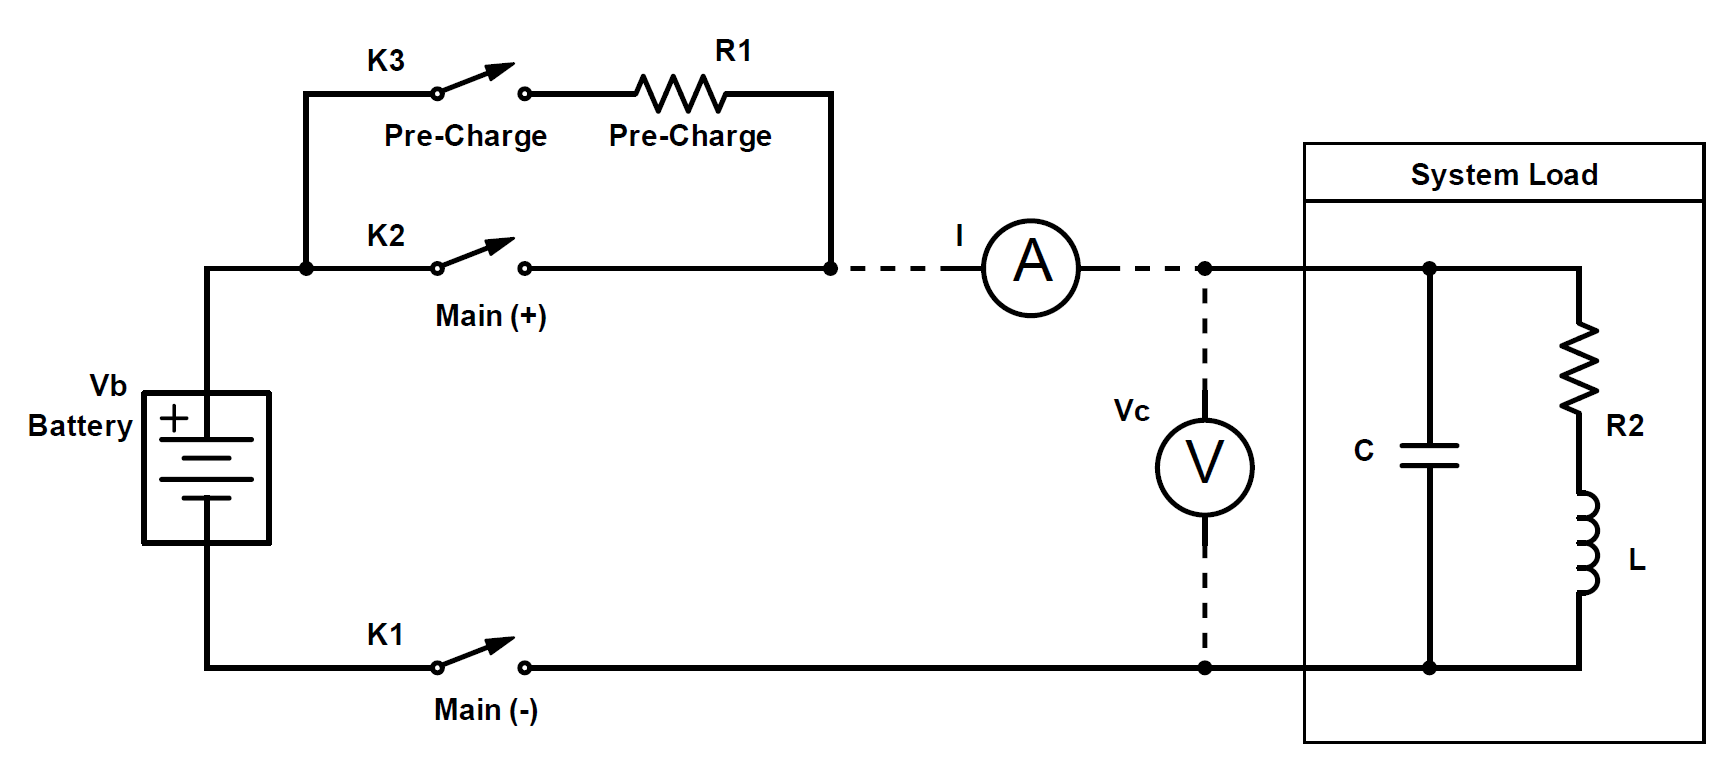
\includegraphics[width=0.7\textwidth]{Images/Implementation/precharge_basics.png}
            \caption{Typical precharge circuit \cite{munari2020precharge}.}
            \label{fig:precharge}
        \end{figure}

        This strategy ensures that the initial charging current is limited by design, significantly reducing electrical stress on the contactors and load, therefore improving system reliability. Once the precharge phase is completed, the resistor is removed from the current path, ensuring that no additional conduction losses are introduced during normal operation.

    \subsection{Design}

        The precharge process can be modelled as an RC charging circuit, where the load capacitance is gradually charged through a series resistance. The voltage across the capacitor during the precharge phase is given by:

        \begin{equation}
        V_c(t) = V_s \left(1 - e^{-t/RC}\right)
        \label{eq:vcap}
        \end{equation}

        Combining Equation~\ref{eq:vcap} with Equation~\ref{eq:current_cap}, the instantaneous current during the precharge process can be expressed as:

        \begin{equation}
        i(t) = \frac{V_s e^{-t/RC}}{R}
        \end{equation}

        These expressions show that both the current and voltage evolution are governed by the time constant $\tau = RC$, which directly determines the precharge duration and the peak inrush current. After one time constant ($t = \tau$), the current decreases to approximately 36.7\% of its initial value, while the capacitor voltage reaches approximately 63.2\% of the final value, as illustrated in Figure~\ref{fig:precharge2}.

        \begin{figure}[!ht]
            \centering
            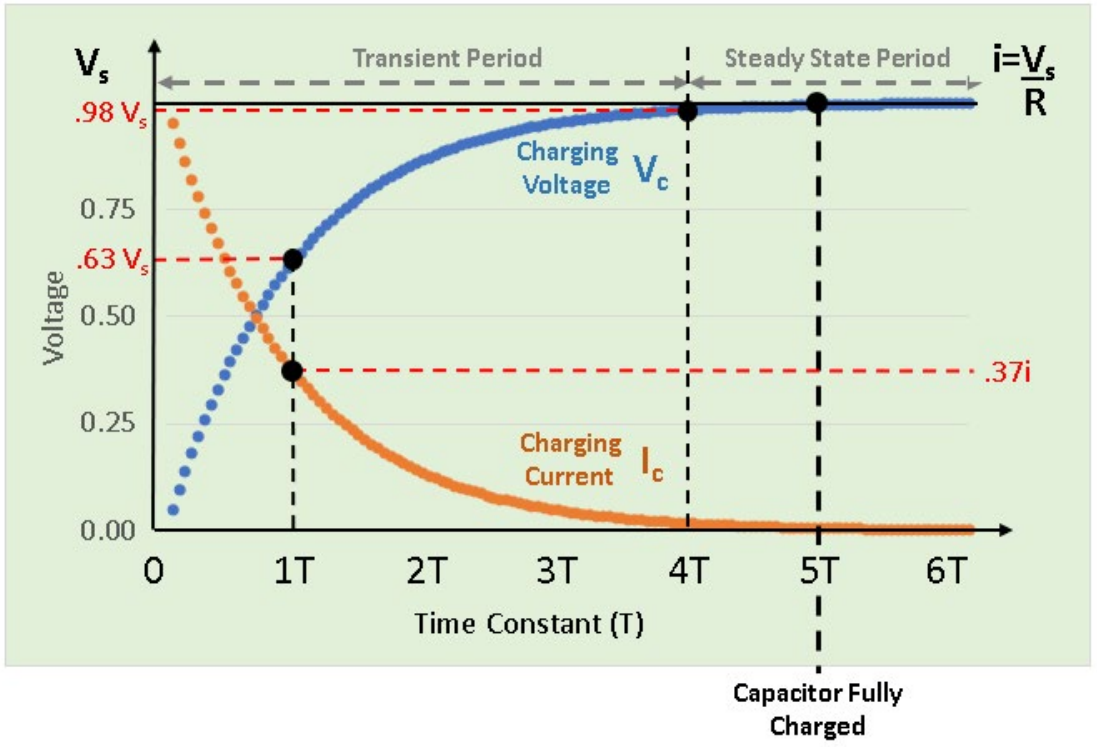
\includegraphics[width=0.5\textwidth]{Images/Implementation/precharge_curve.png}
            \caption{Precharge current and voltage evolution \cite{munari2020precharge}.}
            \label{fig:precharge2}
        \end{figure}

        The transient period is typically considered to span from $0\tau$ to $4\tau$, during which the capacitor reaches approximately 98.17\% of its final voltage. Beyond this point, the system enters the steady-state region, and at approximately $5\tau$, the capacitor is effectively fully charged (99.33\%), although the charging process is asymptotic and never reaches exactly 100\%.

        In practical implementations, the switching between precharge and normal operation is typically performed after approximately $4\tau$ to minimise stress on the contactors while ensuring a sufficiently high load voltage.

        Based on this criterion, the resulting inrush currents can be estimated as:

        \begin{equation}
        I_{inrush}(1\times MPPT) = \frac{50.4 - 50.4 \cdot 0.9817}{0.046} = 20.05~A
        \end{equation}

        \begin{equation}
        I_{inrush}(4\times MPPTs) = \frac{50.4 - 50.4 \cdot 0.9817}{0.016} = 57.65~A
        \end{equation}

        To achieve the desired precharge threshold, a differential comparator circuit was implemented using two voltage dividers as inputs. These dividers scale both the battery-side and load-side voltages to a range compatible with the comparator while simultaneously defining the switching threshold corresponding to the target precharge percentage. The implemented circuit is shown in Figure~\ref{fig:precharge_comp}. The precharge threshold can be adjusted by modifying the value of resistor R2.

        \begin{figure}[!ht]
            \centering
            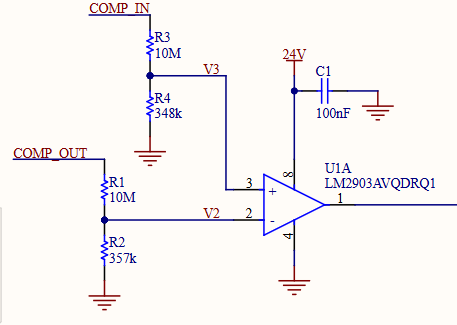
\includegraphics[width=0.5\textwidth]{Images/Implementation/precharge_comp.png}
            \caption{Precharge comparator.}
            \label{fig:precharge_comp}
        \end{figure}

        The remaining circuitry, presented in Appendix~\textcolor{red}{X}, consists of an optocoupler, relays, and the associated control logic implementing the precharge state machine. The system operates through three distinct states:

        \begin{enumerate}
        \item \textbf{System Off:} When either the Battery Management System (BMS) enable signal or the kill switch (KS) is inactive (in the case where the motor controller is the load), all relays remain de-energised, fully isolating the battery from the load.

        \item \textbf{Precharge State:} When both the BMS enable signal and the kill switch are active, the precharge relay (K3) is energised while the main relay remains open. In this state, the load capacitors are charged through the precharge resistor, limiting the inrush current.

        \item \textbf{Normal Operation:} The comparator continuously monitors the voltage difference between the battery side and the load side. Once the load-side voltage reaches approximately 98\% of the battery voltage, the comparator switches state, de-energising the precharge relay (K3) and closing the main relay. The precharge resistor is thereby bypassed, and the system operates under full load voltage conditions.
        \end{enumerate}

        This sequence ensures a controlled energisation of the capacitive load, significantly reducing inrush current and improving the reliability and lifetime of the switching components.

        The precharge duration is primarily determined by the value of the precharge resistor. A higher resistance results in a longer precharge time but lower inrush current, while a lower resistance reduces precharge time at the expense of increased power dissipation. In this design, a $1~k\Omega$ resistor was selected as a compromise between precharge time and power losses, resulting in a precharge duration of approximately 2 seconds, with an average power dissipation of 0.317~W and a peak power of 2.540~W.
        
 
\section{PCB design}
    \subsection{MPPT}
    \label{subsec:PCB_design_MPPT}
        \textcolor{red}{High level explanation of the components and interconections}

        \textcolor{red}{software used, falar sobre o design de 4 layers, pontos de debug, coisas adicionais não faladas anteriormente (pq de cada conector, porta fusiveis, serial to UART, LEDs de debug), posicionamento, segurança adicional de temperatura, dcdcs de power, can, I2C }
        
        
    \subsection{Pre charge}
        The Pre charge \ac{pcb} was designed with the intention of being reusable across other \ac{pcb} systems. For this reason, particular attention was given to achieving a compact and versatile layout. The design uses a two-layer stack-up, as the circuit is relatively simple, which reduces manufacturing complexity and overall cost while still meeting the electrical requirements. The \ac{pcb} is mechanically mounted directly onto the main relay contactors, which simplifies assembly and reduces wiring complexity, Figure~\ref{fig:3D_precharge}.

        \begin{figure}[!ht]
            \centering
            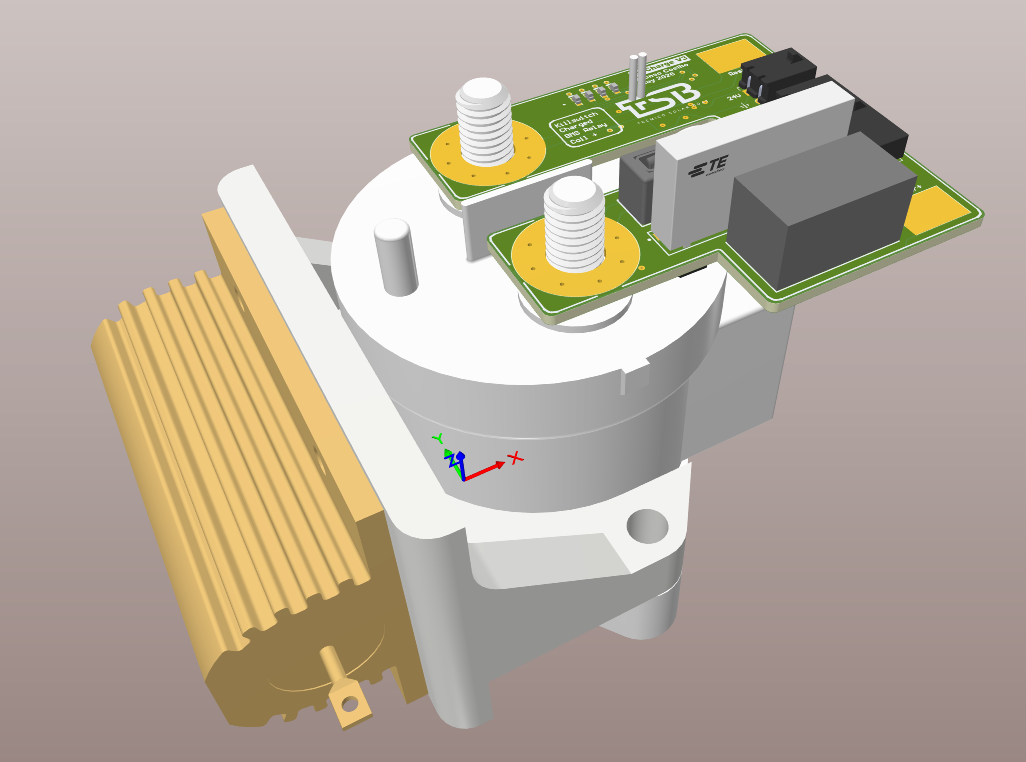
\includegraphics[width=0.5\textwidth]{Images/Implementation/precharge_3D.png}
            \caption{Precharge 3D design.}
            \label{fig:3D_precharge}
        \end{figure}

        In addition, the precharge resistor was intentionally placed outside the \ac{pcb}, mounted to a costume 3D holder. This design choice facilitates easy replacement or adjustment of the resistor value while also contributing to a more compact board footprint. The resistor is electrically connected to the \ac{pcb} by soldering wires directly to dedicated copper pads, ensuring a simple and reliable interface between the external component and the board.

        